\documentclass[a4,oneside,12pt,onecolumn]{extarticle}
\usepackage{style}
\usepackage{pdfpages}

\begin{document}
% Import title page
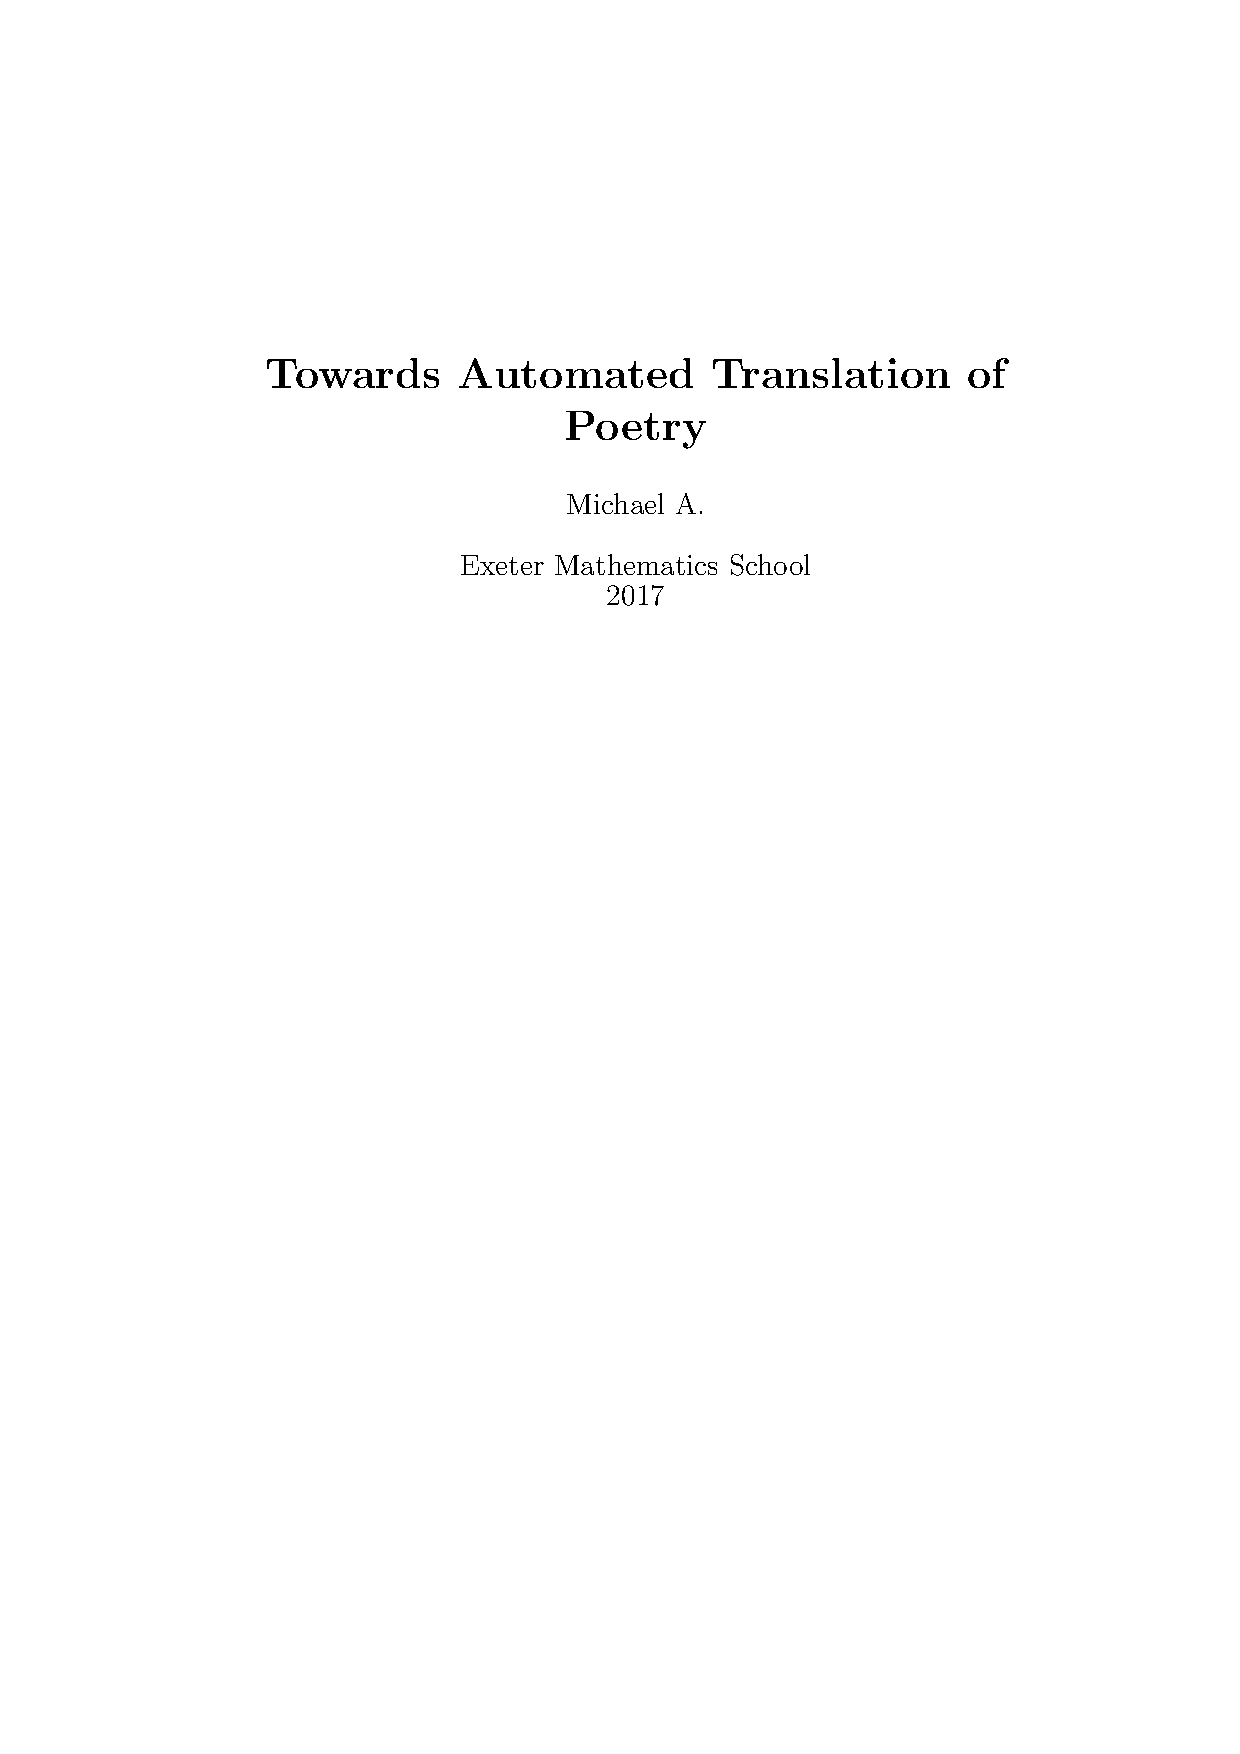
\includepdf[pages={-}]{Title.pdf}
% Above increments page counter by one, so decrement it back 
\setcounter{page}{1}

\begin{abstract}
  \centering\begin{minipage}{0.5\textwidth} As a prerequisite to
    automated machine translation of poetry, I present possible
    methods of improving current word- and phrase-based statistical
    methods to make them more suitable for poetic and literary works.
  \end{minipage}
\end{abstract}

\newpage
\paragraph{}{Translating poetry is hard. Without an intimate knowledge
  of the source and target language, a translation of any text will,
  without a doubt, be lacking. Translating poetry is even harder: and
  to do it computationally, almost impossible. This research project
  explores how we may improve current computational approaches to
  allow for better-quality translations of poetry.}
\paragraph{}{Why would we want to translate poetry? A couple of
  reasons come to mind, which specifically motivated my interest in
  this problem:}
\begin{itemize}
\item Foreign-language poems translated to English have historically
  built up the rich tapestry of English literature: where would we be
  without Dante, Virgil, Homer?
\item Machine translation could be used to translate poems to and from
  languages which have small, if any, translation communities.
\item A faithful translation requires the translator to have intimate
  familiarity with both the source and target languages: a computer
  could do one of these jobs, allowing for a lighter cognitive load on
  the translator and perhaps a better-quality translation.
\item Translated poems are often worth reading for their own merits,
  and it would be an interesting creative exercise to analyze machine
  translated poems.
\item The hope that a more computational, quantitative treatment of
  poetry and poetic analysis will encourage the more
  scientifically-minded to explore poetry and the beauty contained
  therein.
\end{itemize}
%%% Local Variables:
%%% mode: latex
%%% TeX-master: "Poster"
%%% End:

\section*{Background}
\quot{Prose: words in their best order; \\poetry: the best words in
  the best order}{Samuel Taylor Coleridge}

\paragraph{}{Computational linguistics (or Natural Language
  Processing, NLP) is defined by the Association for Computational
  Linguistics as: `the scientific study of language from a
  computational perspective' \cite{acl-def}. The field has its origins
  in the United States, immediately following the Second World
  War. Warren Weaver, an American scientist, wrote a now-famous
  memorandum \cite{weaver} in 1947 to Norbert Wiener at MIT: }
\begin{displayquote}
  I have wondered if it were unthinkable to design a computer which
  would translate. Even if it would translate only scientific material
  (where the semantic difficulties are very notably less), and even if
  it did produce an inelegant (but intelligible) result, it would seem
  to me worth while.
\end{displayquote}
\paragraph{}{Weaver made four core arguments about possible approaches
  to machine translation (MT)\cite{core}:}
\begin{enumerate}
\item The problem of one word having multiple meanings can be solved
  by looking at the $n$ words (or just nouns) around it to
  disambiguate from context.

\item A theorem proved in 1943 by McCulloch and Pitts \cite{pitts}
  suggests that ``a robot\ldots is capable of deducing any legitimate
  conclusion from a finite set of premises''. Under the assumption
  that language is logical, language understanding may be possible.

\item Translation problems can be looked at as a cryptographic
  process: ``a book written in Chinese is simply a book written in
  English which was coded into the `Chinese code','' and cryptographic
  methods can therefore be used to translate text.

\item Instead of translating language-to-language, we should descend
  ``down to the common base of human communication --- the real but as
  yet undiscovered universal language'' to express a concept, then
  express it in the desired language.
\end{enumerate}

\paragraph{}{Weaver's theorems, while not necessarily state-of-the-art
  today, were enough to fuel an increase in interest for language
  processing and machine translation. Most work in the early days was
  military funded: it concerned Russian $\rightarrow$ English (and to
  a minor extent English $\rightarrow$ Russian) translation, intended for use by the
  United States government against the USSR during the Cold War
  \cite{retro}. Its development continued to the mid-1960s, although
  it was strongly confined by the computing power available; systems
  were primarily rule-based, using limited dictionaries. Researchers
  of the famous Georgetown experiment\footnote{A demonstration of
    machine translation in 1954, which translated 60 Russian sentences
    to English with quite astounding accuracy and drew a large amount
    of press attention: however, the methodology was flawed and the
    system was not nearly as impressive as it seemed.} estimated that
  machine translation would be a solved problem in three to five years
  \cite{georgetown}. However, the development was not fast enough: in
  1966 the Automatic Language Processing Advisory Committee (ALPAC)
  published a skeptical report on the future of machine
  translation\cite{alpac}:}
\begin{displayquote}
  At present [MT] serves no useful purpose without postediting
  \textelp{} we will only have adequate mechanical translation when the
  machine can ``understand'' what it is translating \textelp{} perhaps our
  attitude might be different if there were some pressing need for
  machine translation, but we find none.
\end{displayquote}

\paragraph{}{The report did not bode well for NLP research: none of
  its nine recommendations supported any sort of research in MT or NLP
  \cite{alpac-crit}. Research in MT stalled, especially in the
  US. Work began to be done in applying linguistics, rather than raw
  computing power, to problems. A great deal of work was done in
  natural language understanding (for example with
  SHRDLU\cite{shrdlu}). Eventually, by the 1980s, developments in
  corpus linguistics and machine learning began to reawaken the
  slumbering MT community. The focus of research shifted from closed
  to open domains, and from hand-written rules to corpus-based
  statistical approaches \cite{shift}. In 1990, IBM published a
  seminal work in the field, describing progressively more complex
  statistical models for word-based machine translation \cite{ibm}. As
  research boomed, so too did commercial usage of MT systems: the most
  famous examples of which being SYSTRAN (used by the US Department of
  Defense) and METEO (used for English-French weather bulletin
  translation in Canada). }

\paragraph{}{The fields of machine translation and computational
  linguistics continue to grow today. Most major technology companies
  (Apple, Google, Facebook, etc.) have dedicated research departments
  for computational linguistics. Some uses are ubiquitous: Siri,
  Google Translate, Cortana. The rapid pace of development is
  underscored by the speed and scale of improvements in related fields
  such as machine learning. Some of today's most advanced methods of
  machine translation come close to achieving human-level accuracy in
  translation tasks \cite{gnmt}.}

\paragraph{}{But, machine translation is still mostly used for
  translating non-fiction text like scientific papers or newspaper
  articles. So why do we want to translate poetry? A couple of reasons
  come to mind, which specifically motivated my interest in this
  problem:}
\begin{itemize}
\item Translated poems have historically built up the rich tapestry of
  English literature: where would we be without Dante, Virgil, Homer?
  The ability to computationally translate poems may allow yet more
  foreign poems to enter the consciousness of the English language
  \cite{hist}.
\item Furthering the previous point, there are many poems written in
  languages which do not have an active, or for that matter any,
  translation community. Machine translation techniques could be used
  to translate these poems where humans cannot.\footnote{For
    discussion of machine translation for resource-poor languages, see
    Nakov \& Ng (2014) \cite{ng}, Avramidis \& Koehn (2008).
    \cite{avr}}
\item Some argue that a truly faithful translation requires the
  translator to have intimate familiarity with both the source and
  target languages \cite{fam}: if a computer could do the job of being
  familiar with one of the languages, it would lighten the cognitive
  load on the translator and perhaps allow for a better-quality
  translation.
\item Translated poems are often worth reading in their own right:
  ``when translator and original are in tune\ldots a third poem is
  created'' \cite{hist}; indeed, it would be an interesting creative
  exercise to analyze the poems which result from machine translation.
\item The hope that a more computational, quantitative treatment of
  poetry and poetic analysis will encourage the more
  scientifically-minded to explore poetry and the beauty contained
  therein.
\end{itemize}

%%% Local Variables:
%%% mode: latex
%%% TeX-master: "Report"
%%% End:

\section*{Theory}
\quot{How tired I am of stories, how tired I am of neat little phrases \\
  that come down so beautifully with all their feet on the
  ground!}{Virginia Woolf}
\paragraph{A cognitive model of language}{Before we can begin to
  discuss computational approaches to language modeling, it is best
  that we take a moment to discuss cognitive models of language:
  essentially, a way of trying to approximate and describe human
  cognitive (thinking) processes. For all that humans are very good at
  learning and speaking languages --- both as children and adults ---
  we really have no idea {\it why} we're so good at it. As early as
  Roger Bacon's 1245 work `Overview of Grammar' \cite{bacon},
  linguists (or philosophers and grammarians, as they were called in
  those days) have suggested that all languages are built upon a
  common cognitive grammar: that is, human languages are an innate
  experience. Noam Chomsky formalized the idea of a `universal
  grammar' in 1965: \cite{ug} the idea that there is an innate
  language faculty in humans that `knows' the rules that allow for
  language to be developed and used, for example distinguishing nouns
  from verbs. But exactly what this universal grammar is, is not a
  question which has been answered yet.}
\paragraph{}{At multiple points throughout the history of NLP,
  researchers have tried to computationally emulate this internal
  grammar structure, especially within the context of machine
  translation. It stood to reason that if we could build a
  computational grammar good enough, machine translation would become
  easy --- in a similar way to how Weaver suggested we use the
  ``universal language''. The simplest of these attempts were
  rule-based machine translation systems (RBMT), which came in three
  groups: \cite{jur}}
\begin{enumerate}
\item Direct systems, or dictionary-based machine translation, which
  consisted purely of dictionary lookups.
\item Transfer systems, which broke translation up into three steps:
  \begin{enumerate}
  \item Analysis of the source language input to find its grammatical
    structure by, for example, morphological analysis (classifying
    each word as eg. noun, verb, as well as gender, tense, etc), or
    word-sense disambiguation;
  \item Transfer of the resulting structure into a structure useful
    for the target language; and
  \item Generation of text in the target language from the final
    structure.
  \end{enumerate}
\item Interlingua systems, which converted source input to an
  intermediate language-independent representation, then converted
  that to the target language.
\end{enumerate}

\paragraph{}{For all that these approaches became very popular in the
  MT community, they did have some major problems. Rule-based systems
  work reasonably well for closed domains (where you know roughly what
  format your input and output must take, like in the case of METEO),
  but when it comes to open systems (where the input and output could
  be anything), the amount of work needed to maintain complex rules,
  including accounting for ambiguity and idiomatic expressions,
  quickly becomes insurmountable.}

%%% Local Variables:
%%% mode: latex
%%% TeX-master: "../Report"
%%% End:

\paragraph{A statistical model of language}{All these
  rule-based, computational models of cognitive grammar are bound to
  be incomplete: simply put, we do not yet have enough knowledge of
  how the brain interprets and creates language --- what internal
  structures it uses, and so forth --- to be able to express these
  methods and structures computationally. So we compromise. Natural
  language processing and generation (of the kind needed in machine
  translation) doesn't require fully emulating human use of language:
  it only needs to approximate it, mimic it in such a way that it
  seems close to indistinguishable from the real thing. A good way of
  doing this is a probabilistic approach.}
\paragraph{}{The best way to explain the probabilistic model is in
  context: so let's take a look at the statistical model of machine
  translation. Say we want to translate a foreign sentence $f$ into an
  English sentence $e$. Then, by a probabilistic model\cite{smt}, we
  want our translation engine to maximize the probability that a given
  English sentence is the correct translation of the foreign sentence:
  that is, maximize $ \Pr(e|f) $. Intuitively, we can interpret this
  probability as the probability a translator will produce $e$ in the
  target language when presented with $f$ in the foreign
  language.\cite{ibm}}
\paragraph{}{Modeling this probability distribution is difficult: we
  can simplify the problem by applying Bayes' theorem\cite{bayes}: by
  Bayesian decomposition, we can rewrite $\Pr(e|f)$ as:
  $$ \Pr(e|f)=\frac{\Pr(e)\Pr(f|e)}{\Pr(f)}$$ Note that the
  denominator $\Pr(f)$ does not depend on $e$, and so is the same for
  all possible values of $e$: therefore we can just simplify our
  equation to be: $$ \Pr(e|f)= \Pr(e)\Pr(f|e)$$ This gives us two new
  variables to maximize: $\Pr(e)$, the {\it language model}, and
  $\Pr(f|e)$, the {\it alignment model}.}

%%% Local Variables:
%%% mode: latex
%%% TeX-master: "../Report"
%%% End:

\paragraph{Corpuses}{But before we can start, we need to acquire a
  corpus. A corpus, roughly speaking, is just a collection of text in
  our target language. It can come from any source, and indeed corpora
  used in linguistics vary widely: examples include the British
  National Corpus (consisting of 100 million words, covering British
  English in the late 20th century), Brown Corpus (1 million words,
  and tagged for parts-of-speech), and Google Books N-Gram corpus
  (multilingual, and searchable online).}
\paragraph{}{Within machine translation, we need two types of corpus:
  a monolingual (language model) corpus, and a parallel bilingual
  corpus. When looking for a corpus to use, the most important thing
  to consider is the domain and topic of the text. For machine
  translation, the domain and topic of the corpus should, as closely
  as possible, match the domain and topic of the text to be
  translated. So, for example, if we were to be translating scientific
  documents, then the best choice for a corpus to learn from would be
  a corpus of other scientific documents.  In an ideal world, to
  translate a given poem, we'd have: a monolingual corpus, entirely
  consisting of poems in the target language in the same style as our
  poem to translate; and a bilingual corpus of poems in the source
  language, of the same style as our input poem, translated by
  professionals into the target language. However, that does throw up
  some problems, which will be discussed later. }

\paragraph{Sentence alignment}{Once we have acquired a parallel corpus
  to work with, we still need to perform sentence alignment. When a
  human translator translates some text, they do not necessarily
  translate it word-for-word or sentence by sentence: this is
  especially true for languages where the writing system does not
  distinguish sentence boundaries. By aligning sentences within a
  corpus, we can more easily find word and phrase pairs when building
  our alignment model.}

\paragraph{}{Formally, \cite{smt} given a set of sentences in a
  foreign language $f = f_1, f_2 \dots f_{n_{f}}$ and their
  translations into English $e = e_1, e_2 \dots e_{n_{e}}$, we want to
  find a sentence alignment $S = \{ s_1, s_2 \dots s_n\}$ such that
  all sentences in both the source and target language are present
  within the alignment, and each sentence only occurs in one sentence
  pair. The simplest way to do this is with the Gale-Church sentence
  alignment algorithm. \cite{gale} The intuition behind their
  algorithm is that longer sentences in one language tend to be
  translated to longer sentences in the other language, and
  vice versa. A probabilistic score is assigned to sentence pairs
  based on both the ratio of character lengths in the sentences, and
  the variance of this ratio. Then a dynamic programming framework is
  used to find the most likely sentence alignment.}
\paragraph{}{Two steps are required for this algorithm: first,
  paragraphs of parallel text are aligned, then sentences within each
  paragraph are aligned. Paragraph alignment is reasonably easy, as
  paragraphs are almost always already aligned in translated text, and
  tend to be very clearly marked out. This means that they can be
  aligned automatically, with the output being corrected by hand if
  needed.}

\paragraph{}{First we define a distance function $d$ which allows for
  sentence insertion, deletion, and substitution, which takes four
  arguments, $x_1, y_1, x_2, y_2$. We let:\cite{gale}}
\begin{enumerate}
\item $d(x_1, y_1, 0, 0)$ be the cost of substituting $x_1$ with
  $y_1$,
\item $d(x_1, 0, 0, 0)$ be the cost of deleting $x_1$,
\item $d(0, y_1, 0, 0)$ be the cost of inserting $y_1$,
\item $d(x_1, y_1, x_2, 0)$ be the cost of combining $x_1$ and $x_2$
  to make $y_2$,
\item $d(x_1, y_1, 0, y_2)$ be the cost of expanding $x_1$ to $y_1$
  and $y_2$
\item $d(x_1, y_1, x_2, y_2)$ be the cost of merging $x_1$ and $x_2$
  and matching with $y_1$ and $y_2$
\end{enumerate}

\paragraph{}{Then we can use a dynamic programming algorithm to align
  the sentences, defined as follows:\cite{gale}}
\begin{displayquote}
  Let $s_i$, $i=1 \dots I$, be the sentences of one language, and
  $t_j$, $j=1 \dots J$ be the translations of those sentences in the
  other language. Let $d$ be the distance function defined previously,
  and let $D(i, j)$ be the minimum distance between sentences
  $s_1 \dots s_i$ and their translations $t_1 \dots t_j$, under the
  maximum likelihood alignment. $D(i, j)$ is computed by minimizing
  over six cases (substitution, deletion, insertion, contraction,
  expansion, and merger) which, in effect, impose a set of slope
  constraints. That is, $D(i, j)$ is defined by the following
  recurrence with the initial condition $D(i, j) = 0$:\\
  $$
  D(i, j) = \text{min}
  \begin{cases}
    D(i, j-1)   &+ \quad d(0,   t_j, 0,       0)       \\
    D(i-1, j)   &+ \quad d(s_i, 0,   0,       0)       \\
    D(i-1, j-1) &+ \quad d(s_i, t_j, 0,       0)       \\
    D(i-1, j-2) &+ \quad d(s_i, t_j, 0,       t_{j-1}) \\
    D(i-2, j-1) &+ \quad d(s_i, t_j, s_{i-1}, 0)       \\
    D(i-2, j-2) &+ \quad d(s_i, t_j, s_{i-1}, t_{j-1}) \\    
  \end{cases}
  $$\\
\end{displayquote}
%%% Local Variables:
%%% mode: latex
%%% TeX-master: "../Report"
%%% End:

\paragraph{Language model}{With a language model, we can assign a
  probability to a sequence of words. Intuitively, the sentence `the
  house is small' \cite{smt} should be more likely than `small the is
  house'.\footnote{However, to quote Chomsky: ``It must be recognized
    that the notion `probability of a sentence' is an entirely useless
    one''. The probability of a sentence has no intrinsic linguistic
    meaning, because humans do not produce language on a statistical
    basis.} We can use a statistical language model to accurately
  describe just how much more likely it is. To build our language
  model, we take a single-language corpus and use $n$-grams by way of
  the Markov assumption\cite{markov}, in a similar way to Weaver's
  original suggestions.}
\paragraph{}{Let's say that we want to estimate the probability of a
   sequence of words, $W = w_1, w_2, \dots w_n$. The na{\"i}ve
   approach to this would be to take a sufficiently large corpus,
   count how many times $W$ appears in it, and divide by the total
   number of $n$-word sequences to get a probability for $W$: however,
   even for an extremely large corpus, it is very unlikely that $W$
   will have appeared at all in its exact form, making probability
   distributions extremely sparse. What we can do instead is use the
   chain rule to decompose the probability of $W$\cite{smt}:
   $$ \Pr(w_1, w_2, \dots w_n) = \Pr(w_n | w_1 \dots w_{n-1})$$ This
   is still cumbersome to calculate, so we can restrict our
   calculations to only a history of words, that is
   $$ \Pr(w_n | w_1 \dots w_{n-1}) \approx \Pr(w_n|w_{n-m} \dots
   w_{n-1})$$ We use the Markov assumption here by saying that only a
   limited number of previous words affect the probability of the
   $n$th word.\footnote{While this assumption is technically wrong,
     it is a convenient simplification, because shorter word histories
     have less sparse probability distributions.} Most commonly,
   language models will restrict their search space to the previous
   two words (called {\it trigrams}, because they consider sets of
   three words) or just the previous word (correspondingly called {\it
     bigrams}). Expanding the search space for larger values of $n$ is
   usually a matter of diminishing returns. }
 \paragraph{}{If we therefore wanted to estimate the probability of a
   given trigram consisting of the sequence $T = w_1, w_2, w_3$, we would 
   count the amount of times we see the sequence $w_1, w_2, w_3$ in
   the corpus, and divide it by the amount of times we see just the
   sequence $w_1, w_2, x$ for all words $x$: that is, we divide the
   count of that specific trigram by the count of all trigrams which
   start with its history. Then by maximum likelihood estimation
   \cite{smt}, the probability of $T$ is therefore:
   $$ \Pr(T) = \frac{\text{count}(w_1, w_2, w_3)}
   {\sum_x \text{count} (w_1, w_2, x)}$$ \\The formula for a general
   $x$ is defined similarly. We can calculate this for all occurring
   $n$-grams in a corpus to give us an $n$-gram probability
   distribution for that corpus. }
 \paragraph{}{It is worth noting at this point that these resulting
   probabilities are not (and should not be!) used as they are:
   $n$-gram models are very sensitive to the training corpus
   \cite{jur}, and as such we have two issues: sparse data
   (probabilities for most $n$-grams will generally be quite low, by
   Zipf's law \cite{zipf}, and will be zero for $n$-grams not seen in
   the training corpus), and how to deal with out-of-vocabulary (OOV)
   tokens (any $n$-gram containing a word not seen in the training
   corpus will have a probability of 0). To deal with OOV tokens, we
   can either simply insert an `unknown' token (usually `UNK') into
   the training data, or we can replace the first occurrence of each
   vocabulary word with `UNK', and then calculate its probability
   distribution in the same manner as any other word. The best method
   of dealing with the sparse data issue is by using smoothing
   methods: these allow us to get better estimates for $n$-grams which
   occurred rarely in the training data, or not at all. There are
   numerous methods, which I will not go into here, including
   Kneser-Ney Smoothing and Good-Turing estimation. Backoff and
   interpolation methods may also be used\cite{jur}. }

%%% Local Variables:
%%% mode: latex
%%% TeX-master: "../Report"
%%% End:


 \paragraph{Alignment model}{How we approach our alignment model
   depends on if we are using {\it word-based} or {\it phrase-based}
   machine translation.\cite{smt}}
 \paragraph{Word-based}{While word-based models are no longer
   state-of-the-art, the methods which are used for them remain
   relatively applicable to modern MT problems, as well as being
   interesting in their own right. The following section will be based
   on the IBM models of machine translation first presented in 1990
   \cite{ibm}, which are still used to an extent in the GIZA and
   GIZA\texttt{+}\texttt{+} toolkits for alignment. Word-based models,
   are, predictably, based on translating words in isolation, or {\it
     lexical translation}. Firstly, we take a corpus of texts in a
   foreign language, and their translations into English, and then
   calculate statistics (a lexical translation probability
   distribution) from these.}
 \paragraph{}{Formally speaking, we want to calculate the probability
   that a given foreign word $f$ translates into a given English word
   $e$, given the data in our corpus. The most straightforward way of
   doing this is, again, maximum likelihood estimation: we take the
   count of the amount of times we see $f$ translated to $e$, and
   divide it by the amount of times we see $f$ overall in the
   corpus. Smoothing can again be used here to account for data
   sparsity and OOV tokens.}
 \paragraph{}{Given this probability distribution, we can now get to
   the task of building our alignment model. A foreign sentence $F$
   can be translated to an English sentence $E$ by use of an
   alignment: a mapping of foreign words to English words. We
   can map this using an alignment function, which may allow for
   adding, removing, and duplicating words: in this case, each English
   word must be linked to exactly one input word, which may be a
   special NULL token. On the other hand, one input word may be linked
   to multiple output words, or none at all. \cite{smt}}
 \paragraph{}{The IBM Model 1 is a generative model (meaning it breaks
   the problem up into smaller steps, and then generates a final
   answer using these intermediate steps), and is based only on the
   aforementioned lexical translation probability distribution. It is
   described in quite some detail in Brown et al. (1993) \cite{m1}, so
   I will only give a superficial gloss. In short, the IBM Model 1
   defines the probability of translating a foreign sentence
   $f = f_1, f_2 \dots f_n$ of length $l_f$ into an English sentence
   $e = e_1, e_2 \dots e_n$ of length $l_e$, with an alignment of each
   English word $e_j$ to a foreign word $f_i$ according to the
   alignment function $a(j) = i$. The formula to calculate this probability is:
   $$ \Pr(e, a|f) =
   \frac{\epsilon}{(l_f + 1)^{l_e}} \prod_{j=1}^{l_e}t(e_j|f_{a(j)})$$
   where the leading fraction is used to normalize the distribution so
   all probabilities are between 0 and 1, and $t(e_j|f_{a(j)})$ is the
   probability of a given English word being translated into its
   aligned foreign word, from our earlier lexical translation
   probabilities. }
 \paragraph{}{Higher IBM Models increase in complexity and improve
   upon the first model's flaws; in short, they are \cite{smt}:}
 \begin{itemize}
 \item Model 1: lexical translation, as discussed above.
 \item Model 2: adds an explicit alignment model, which allows for a
   more statistically likely alignment.
 \item Model 3: adds a fertility model, which estimates the amount of
   output words that a foreign word `produces', allowing for input
   words to be dropped (eg. flavoring particles), and a distortion
   probability, which allows for more reordering in
   translation.\footnote{In practice, the Model 3 is sufficient for
     modern uses: using any models after this is superfluous.}
 \item Model 4: adds a relative alignment model, which fixes issues
   with Model 3's distortion model by looking at relative distortions
   instead.
 \item Model 5: fixes issues with previous models where multiple
   output words could be placed in the same positions, which wasted
   probability mass.
 \end{itemize}


 \paragraph{Phrase-based}{Phrase-based models are widely considered as
   state-of-the-art today \cite{smt} and outperform word-based models
   by a large margin \cite{koehn}. As the name suggests, they are
   based on phrases (short sequences of words), and processing is done
   on these phrases. The motivation behind this is clear to speakers
   of foreign languages: in many cases, a word in one language cannot
   be easily translated to another language because it has
   phrase-specific meanings. Phrase-based translation segments an
   input sentence into phrases, translates those phrases, and reorders
   them as needed. This has multiple advantages compared to the
   word-based model: it allows for one-to-many and many-to-one
   mappings, resolves translation ambiguities, and is conceptually
   much simpler. \cite{smt}}
 \paragraph{}{We start with exactly the same base equation as for word
   based models: that is, we look to maximize
   $$ \Pr(e|f) = \Pr(f|e)\Pr(e)$$ However, for the phrase-based model,
   we further decompose $\Pr(f|e)$ into phrase translations\cite{smt}:
   $$ \Pr(\bar{f}_1^I | \bar{e}_1^I)  =
   \prod_{i=1}^j \phi(\bar{f}_i | \bar{e}_i) \ d(\text{start}_i -
   \text{end}_{i-1} - 1)$$ We break up each foreign sentence $f$ into
   some $I$ phrases $\bar{f}_i$, and the same for each English
   sentence; each segmentation of phrases is equally likely. $\phi$ is
   a mapping of the probability of each English phrase being
   translated into a foreign sentence. The distance model $d$ is used
   to reorder the phrases.}
 \paragraph{}{Splitting a sentence into phrases can be done using a
   word alignment, like those seen in the earlier word-based
   translation section. We collect all aligned phrase pairs that are
   consistent with the word alignment. A phrase pair ($\bar{f}$,
   $\bar{e}$) is {\it consistent} with an alignment $A$ if all words
   in $\bar{f}$ with alignment points in $A$ have corresponding
   alignment points with words in $\bar{e}$, and vice versa: as a
   result, the words in a consistent phrase pair are only aligned with
   each other, and not to words outside that phrase
   pair.\footnote{This can leave us with phrases which are
     non-intuitive, for example `house the`: interestingly, pruning
     out these non-intuitive, syntactically incorrect pairs actually
     can decrease the performance of a model.\cite{koehn}} We can then
   estimate the phrase translation probability distribution in much
   the same way as we estimate $n$-gram probabilities, as
   $$ \phi(\bar{f} | \bar{e}) =
   \frac{\text{count}(f, \bar{e})}
   {\sum_{\bar{f}}\text{count}(\bar{f}, \bar{e})}$$ }
 \paragraph{}{The reordering of our English phrases, relative to the
   input foreign phrases, is done by the relative distortion
   probability function $d(s_i - e_{i -1})$, where $s_i$ is the start
   position, in terms of words, of the foreign phrase which was
   translated to the $i$th English phrase, and $e_{i-1}$ is the end
   position of the foreign phrase translated to the ($i-1$)th English
   phrase. For simplicity, $d$ is modeled by an exponentially decaying
   cost function, $d(x) \approx \alpha^{|x|}$, for some value of
   $\alpha$, $ 0 \leq \alpha \leq 1$, so larger distortions are much
   less probable, although some work has been done on modeling
   distortion using joint probability distributions \cite{wong}.}

%%% Local Variables:
%%% mode: latex
%%% TeX-master: "../Report"
%%% End:


%%% Local Variables:
%%% mode: latex
%%% TeX-master: "Report"
%%% End:

\section*{Discussion}
\quot{What is translation? On a platter \\ A poet's pale and glaring
  head}{Vladimir Nabokov}
\paragraph{}{Following the heavy math of the previous section, I
  return here to the crux of the problem: poetry, and translating
  it. To dig into the meat of the problem, let's consider an exemplar
  poem, and how we might approach translating it, both by hand and
  computationally. }

\paragraph{}{Vladimir Nabokov, in the notes of his controversial
  translation of Aleksandr Pushkin's work `Eugene Onegin'
  \cite{nabokov, nabokovtheory}, argues that all translations of poetry will
  inevitably fall under three categories:}
  \begin{description}
  \item [Paraphrastic] A free version of the original: words and
    phrases are toyed with --- added, removed, or changed --- in order
    to conform to some form that the translator wishes.
  \item [Lexical] Translating the basic meaning of words and their
    order.
  \item [Literal] Translating as closely as possible the original,
    with the exact contextual meaning being preserved.
  \end{description}

  \paragraph{}{Nabokov believed that only the final item, literal
    translation, was a `true' translation, and all others only served
    to tarnish the poem:}
  \begin{displayquote}
    The hack who has never read the original, and does not know its
    language, praises an imitation as readable because easy platitudes
    have replaced in it the intricacies of which he is unaware.
  \end{displayquote}
  \paragraph{}{Nabokov's translation of `Eugene Onegin', predictably,
    fell into the `literal' camp of translation. The original poem
    consisted of stanzas of iambic tetrameter, with the rhyme scheme
    `AbAbCCddEffEgg'. Note that uppercase letters represent
      feminine rhymes (a rhyme which matches two or more syllables, in
      which the final syllables are unstressed), and lowercase letters
      represent masculine rhymes (a rhyme with matches only one
      syllable, which is stressed). Nabokov argued that ``to
    reproduce the rhymes and yet translate the entire poem literally
    is mathematically impossible'', and as such decided to eschew
    translating the rhyme scheme: his final version contained no
    rhymes, but translated meticulously every word of vocabulary and
    every structural choice which Pushkin made while writing the poem,
    as well as containing extensive commentary. It is considered the
    most `faithful' translation of the original, and it serves as a
    useful gloss for those wanting to read the original poem, but not
    possessing a suitable level of Russian.  }

  \paragraph{}{With these three options in mind, let's explore the
    manual and computational approaches one may take to translating
    what is considered to be one of the most beautiful works in the
    German language\cite{goethe}: Goethe's `{\"U}ber allen Gipfeln'
  \footnote{Also called `Wanderer's Nightsong II', as it is the
      second part of Goethe's `Wandrers Nachtlied' series. } Here is
    the text of the original: \\}

% Hacky fix, needs to stay on one line
\begin{minipage}{0.8\linewidth}
  \begin{verse}

    {\"U}ber allen Gipfeln \\
    Ist Ruh, \\
    In allen Wipfeln \\
    Sp{\"u}rest du \\
    Kaum einen Hauch; \\
    Die V{\"o}gelein schweigen im Walde. \\
    Warte nur, balde \\
    Ruhest du auch.
  \end{verse}
  \attrib{Johann Wolfgang von Goethe (1749--1832)}
\end{minipage}

\paragraph{}{Firstly, let us consider a lexical translation --- that
  is, a translation which considers only the basic preservation of
  words and their order. The following gloss was done using an
  English-German dictionary, with alternative words marked using
  slashes: \\}

% \begin{minipage}{0.8\linewidth}
  \begin{verse}
    Over all peaks\slash summits\slash tops \\
    Is rest\slash peace\slash silence, \\
    In all treetops \\
    You (informal) sense\slash feel \\
    Hardly a breath\slash breeze; \\
    The little birds remain silent\slash keep still in the wood\slash forest. \\
    Just wait, soon \\
    You rest\slash repose too\slash also. \\
  \end{verse}
  \attrib{TU Chemnitz Dictionary\cite{beo}}
% \end{minipage}

  \paragraph{}{Doing this by hand only requires a bilingual dictionary
    and knowledge of the target language: as such, a computational
    approach would, at most, require access to a good English-German
    dictionary. This is, then, the simplest computational approach,
    requiring no large amounts of mathematics or programming. Note how
    the rhyme scheme has not been preserved, excepting the duplication
    of `tops' in lines 1 and 3,\footnote{While this is technically a
      rhyme, a poet using a word as its own rhyme is committing a
      crime against poetry.} or the half-rhyme of peaks-peace in lines
    1 and 2. Looking at preservation of rhythm is pointless, because
    the translation purposely sacrifices ease of reading for
    completeness of translation: it would not make sense to read this
    poem aloud.\footnote{Unless one is E.E. Cummings, in which case it
      is fine.}}

\paragraph{}{Next, consider what Nabokov would have called the
  paraphrastic version: John Whaley's translation, which hangs on a
  plaque in a reproduction of the cabin where Goethe wrote the
  original poem: \\}

\begin{minipage}{0.8\linewidth}
  \begin{verse}
    Over all of the hills \\
    Peace comes anew, \\
    The woodland stills \\
    All through; \\ 
    The birds make no sound on the bough. \\
    Wait a while, \\
    Soon now \\
    Peace comes to you. \\
  \end{verse}
  \attrib{John Whaley}
\end{minipage}

\paragraph{}{Let us consider which parts of the original poem this
  translation preserves, and which parts it changes. The rhyme scheme
  of the original is {\it ababcddc}; the translation, on the other
  hand, is {\it ababcdcb} --- so the rhyme scheme has been preserved
  to an extent. But to allow for this preservation of rhyme scheme,
  the poem has been altered in a way that would disgust Nabokov. The
  first line is translated in the same way. The second line goes from
  `is peace' to `peace comes anew' --- a change in tense which is only
  done to allow a rhyme two lines later. The rest of the poem has been
  completely altered: it goes from `in all treetops, you feel hardly a
  breath' to `the woodland stills all though'; the birds move from the
  forest to the bough; and instead of you finding peace, the peace
  comes to you.}
\paragraph{}{The original poem is considered one of the most beautiful
  works in the German language, primarily for two reasons. The first
  is the contrast Goethe draws between man and nature: man is
  restless, uncomfortable in the silence of the forest but expecting
  of death's eternal peace. On the other hand, nature is united in its
  silence. The scale of the poem is also interesting: it moves from a
  large scale (the summits), to a middle distance (the treetops), to
  the immediate surroundings (in the forest), and finally to the
  person. This sequence can be seen as encompassing the human
  universe, moving from the largest (visible from a forest) scale, to
  the smallest, most personal. The translation of the poem loses the
  large scale (summits turn to hills), although it preserves the progression
  of scale reduction. But man's restlessness is lost: instead of man
  having to wait for eternal peace, it becomes peace coming to man.}
\paragraph{}{Instead of looking at this poem as a translation of
  Goethe's original, it might be better to look at it as a poetic work
  in its own right. Looking at it from that point of view, it is very
  much a good poem. There is a good rhythm, a good rhyme scheme, and
  it reads well: and, while there is not necessarily the same level of
  conciseness and beauty that Goethe's poem shows, it is still a read
  to be savored.}
\paragraph{}{It is worth discussing here the work of Douglas
  Hofstadter in his book `Le Ton Beau de Marot' \cite{hof}. The book
  covers possible translations of the Cl\'{e}ment Marot's `Ma
  Mignonne': by exploring various possible translations, the author
  explores a wide range of topics in linguistics, psychology, and
  mathematical theory. Hofstadter is perhaps the most vocal supporter
  (outside of translation circles) of the paraphrastic approach to
  translation. The book contains a multitude of possible translations
  and transformations of the poem, most of which are barely
  recognizable to be related to the original. They are good reads,
  just as Whaley's translation is a good read. But they do not stay
  faithful to the original. While intended to be a proof of the
  superiority of the paraphrastic approach to translation, what
  Hofstadter's book really shows us is the unsuitability of
  paraphrastic translation to preserving the context and meaning of
  the poem. Instead, it can be seen as proof that paraphrastic
  translation creates a new, distinct poem.  }

\paragraph{}{How would one go about manually taking the literal
  approach to this poem? I believe the task is beyond the scope of
  this report. The main issue is that there is a deep understanding of
  both languages required: Nabokov himself was bilingual in both
  English and Russian from childhood, and thus had the kind of
  intimate understanding of both languages and cultures which I
  simply do not possess. Additionally, there are time constraints:
  Nabokov's own translation took many years of research
  \cite{nabokov}, and the time frame for this project was
  limited. Perhaps one might start with exploring Goethe's background,
  his other poetry, and so on, and explore the area, working and
  reworking a translation in much the same way as the poet might have,
  until a suitably literal translation is reached.}

\paragraph{}{Considering all of the above, what is the best
  computational approach we could take to translate poetry? Manually,
  the best approach, in my opinion, is the literal approach: a
  preservation of the original poem's contextual meaning. A
  computational literal translation can be considered to be under the
  umbrella of `AI-complete' problems. Paraphrastic translation, for
  all Nabokov disparaged it, is a good computational option: while it
  does not preserve the original, it does create a new poem which, as
  seen above, is still worth reading in its own right: it is also
  easier, computationally, to implement.}

\paragraph{}{To get an idea of what we're working with, here is how
  Google Translate, arguably the most popular translation service
  today, translates the poem.\footnote{It must be noted here that as
    of 2016, Google Translate uses neural machine translation for
    English $\leftrightarrow$ German translation, the explanation and
    analysis of which is beyond the scope of this report. I will be
    focusing only on the types of translation I outlined in the theory
    section; nonetheless, analyzing its poetic output is an
    interesting exercise. }\\}

\begin{minipage}{0.8\linewidth}
  \begin{verse}
    Above all peaks \\
    Is peace, \\
    In all tops \\
    Do you feel \\
    Hardly a breath; \\
    The birds are silent in the forest. \\
    wait, soon \\ 
    Are you retiring too? \\
  \end{verse}
  \attrib{Google Translate}
\end{minipage}

\paragraph{}{The first thing to notice about this translation is its
  somewhat perplexing tendency towards converting statements to
  questions. `Sp{\"u}rest du' becomes `do you feel' --- a reasonable
  mistake to make, because the German language does not use an
  auxiliary (`do') to indicate a question: it simply reverses the verb
  and the noun to indicate its presence. However, the following and
  preceding lines make it clear that this is not an isolated phrase,
  which could be interpreted as a question, but rather part of a
  sentence clause. Another interesting thing is the vocabulary
  choices: `Gipfeln' is translated to `peaks', as opposed to the more
  common translation `summits'; the word `nur' is also cut completely,
  which eliminates the feeling of urgency and restlessness which its
  use in the original poem implies.}

\paragraph{}{My research has consisted of hypothesizing changes to
  current (word- and phrase-based) machine translation methods which
  would allow for more fluent poetic output, compared to the type
  shown above. I have developed three
  hypotheses:}
\begin{enumerate}
\item Training the language and alignment models on a poetic corpus
  improves poetic qualities of the output translation.
\item Altering the sentence alignment model for poetic works will
  improve line-by-line translation quality.
\item Poetic characteristics can be preserved by constraints on the
  hypothesis space, or recovered by post-processing of the output
  translation.
\end{enumerate}

\paragraph{Poetic corpus}{I would argue that statistical translation
  of poetry faces the same problem as statistical modeling of
  language: we simply have no way of truly modeling the poet's thought
  processes while writing the original, and therefore no way of
  emulating it computationally. So, again, we have to compromise:
  instead of seeking to emulate the thought process, we instead seek
  to statistically model poetry in such a way that our translation
  sounds poetical. }
\paragraph{}{The primary way of having a `poetic' sounding translation
  is through corpus choices. Google Translate's language and alignment
  models for English $\leftrightarrow$ German translation are
  primarily trained on the Europarl corpus, which is a transcription
  of all European Parliament proceedings, and is available in all the
  official languages of the Parliament \cite{parl}. Multilingual
  corpus availability is a large problem in machine translation, and
  the Europarl corpus is large enough that it can be used as a basis
  for alignment models when translating the applicable European
  languages. However, alignment models, like language models, are
  sensitive to the input corpus (even with smoothing), and will prefer
  alignments with words which occur often in the corpus. Europarl
  proceedings are, predictably, very dry and not at all poetic. A
  non-poetic input implies a non-poetic output. The obvious solution
  here is to use a parallel corpus of German poems and their English
  translations. Unfortunately, no such corpuses exist, and creation is
  extremely difficult, as very few parallel poetic translations are
  available in easily-processable digital form. In an ideal world, to
  translate a given poet's poem, we'd use a corpus of parallel
  translated poems from the same time period or style. Unfortunately,
  this is not the ideal world, so some compromise is needed. }
\paragraph{}{Using a poetic language model is a much more reasonable
  and achievable solution. A suitable language model can be built, I
  believe, simply by collecting a large amount of poetry in the target
  language --- in this case, English, and using this to train the
  language model. As part of this project, I scraped the top 500
  English language works from Project Gutenberg tagged under `poetry'
  and collated them into a corpus, which could possibly be used to
  train a language model with a toolkit that allows it. However, this
  method does raise some problems.}
\paragraph{}{Kao (2011) \cite{kao} showed that there are certain
  characteristics which occur specifically in professionally-written
  poems. The primary features, for modern poetry, are firstly the
  reduced presence of rhyme and alliteration, secondly the use of
  concrete nouns, and thirdly the use of less common
  words. Preservation of these features is well-paired with
  phrase-based machine translation. The lack of rhyme and alliteration
  means we do not need to find ways to parse for them, which is a
  difficult task due to variations in pronunciation. The increased use
  of concrete nouns can be applied by adding an extra weighing to
  these tokens while training our language model. The use of less
  common words is more difficult, as language models, by design, favor
  more common words. A possible solution would be performing extra
  smoothing on the corpus which, for example, greatly increases the
  probability of less common words and decreases the probability of
  more common words. The problem with this, of course, is that less
  common words will begin to be used where a poet may not necessarily
  use them: for example, substituting `to have' with `to possess' or
  `to retain'. }

\paragraph{Alignment model}{Whereas sentences in prose are clearly
  defined, poetry does not have strong sentence distinctions. In some
  cases, a line break may indicate the end of a sentence: in others, a
  line break may indicate the end of a clause, or even just
  nothing. Compare the following extracts of poems:\\}


\begin{minipage}{\linewidth}
  \begin{verse}
    one's not half two. It's two are halves of one: \\
    which halves reintegrating,shall occur \\
    no death and any quantity;but than \\
    all numerable mosts the actual more
    \attrib{ee cummings\cite{cummings}}
  \end{verse}
\end{minipage}

\begin{minipage}{\linewidth}
  \begin{verse}
    Sunlight pouring across your skin, your shadow \\
    >[0.55\linewidth] flat on the wall. \\
    The dawn was breaking the bones of your heart like twigs. \\
    You had not expected this, \\
    >[0.1\linewidth] the bedroom gone white, the astronomical light \\
    >[0.4\linewidth] pummeling you in a stream of fists.
    \attrib{Richard Siken \cite{siken}}
  \end{verse}
\end{minipage}

\paragraph{}{In the first poem, line breaks have no meaning: aside
  from adding a small pause when the poem is read out loud, they can
  completely be disregarded. There are no traditional sentence
  boundaries.  This is an issue with phrase-based translation, as it
  relies on the existence of aligned sentences, and to have aligned
  sentences, one needs clearly defined sentence boundaries. An option
  for this would be to define sentence boundaries as new lines, rather
  than standard punctuation (. !  ?). However, in this case, it would
  lead to important phrases, such as `than all' being split. In
  theory, this shouldn't be an issue --- as already mentioned,
  phrase-based translation actually performs better when
  non-syntactically correct phrase alignments are allowed --- however,
  with translation of meaning in poetry being so context-dependent
  (see the Google Translate example), it could be severely detrimental
  to translation quality. }
\paragraph{}{The second poem is one in which using line-endings for
  separating sentence units would not work: in this case, parsing for
  traditional sentence endings will, in fact, work, because the line
  breaks have only been introduced due to the stylistic preferences of
  the author. The most striking part of this poem is actually the
  layout on the page, which I have tried my best to reproduce from the
  original. A translation would need to reproduce this indentation as
  well, but this could be done quite easily by parsing for whitespace
  at the start of a line in the original poem and using the same
  amount of whitespace in the translation.\footnote{This would only
    work for systems where features like whitespace are not stripped
    before being input.}}
\paragraph{}{A possible solution to the sentence alignment issue would
  be to split poems into two types:}
\begin{enumerate}
\item Poems whose sentences can be treated in the same way as prose,
  where sentences can be assumed to be marked by standard sentence
  boundaries.
\item Poems whose sentence boundaries are marked by line-endings,
  rather than punctuation.
\end{enumerate}
\paragraph{}{The first feature is already used in common sentence
  alignment tools: the second feature could be implemented relatively
  easily by tagging new sentences on line breaks. }

\paragraph{Preserving poetic qualities}{Now that we have dealt with
  the first two problems, we now face the third: how do we preserve
  poetic characteristics while translating? State-of-the-art systems,
  as mentioned already, do not put any weight on preserving aspects of
  poetry such as rhythm or rhyme. There are two possible ways: either
  hypothesis constraints, or post-processing.}
\paragraph{}{Genzel, Uszkoreit, and Och (2010) \cite{genzel} use
  hypothesis constraints to preserve poetic features such as meter,
  line length (syllable and word), or rhyme. By treating poetic
  features as constraints on the poem --- for example, a haiku has a
  constraint on line length and syllable count --- they implement a
  generic poetic form feature function for phrase-based statistical
  machine translation systems. This is a feasible solution to the
  problem of preserving certain poetic features. However, there is an
  issue in the output: while it preserves poetic features, it does not
  preserve fluency, which is of high concern when it comes to
  translating poetry. Here is an example from the paper of a baseline
  translation, and a `couplet in amphibrachic tetrameter' (stressed
  syllables italicized): \\}
\begin{displayquote}
  A policeman said that three people were arrested and that the
  material is currently being analyzed. 
\end{displayquote}
\begin{displayquote}
  An {\it of}ficer {\it sta}ted that {\it three} were ar{\it re}sted \\
  and {\it that} the e{\it quip}ment is {\it cur}rently {\it test}ed.
\end{displayquote}

\paragraph{}{Another solution, instead of searching inside the
  hypothesis space, would be to use post-processing. In many uses of
  machine translation, the output already undergoes post-processing by
  experienced translators or native speakers to fine-tune the output.
  We could, in much the same way, recover poetic features which were
  `lost in translation' by computational post-processing. For example,
  if we wanted to preserve the rhyme scheme of the original poem, it
  could be enough to look for the rhyming synonyms of words at the end
  of lines, and replace those words with their synonyms until the
  lines rhyme in the same way as the original. This is a very
  na{\"i}ve approach, but I believe it could work, given a good enough
  synonym dictionary. There could also be a distortion model, in much
  the same way as phrase-based translation systems, to allow for word
  reordering. This could essentially be seen as implementing a second
  machine translation system, but instead of translating from a
  foreign language to English, we translate from non-poetic to poetic
  English. }

\paragraph{}{What I have assumed while discussing the two previous
  methods is that we already know what poetic features a poem
  has. While it is relatively easy for a trained human to identify and
  annotate such features, it is a non-trivial task for computers to do
  perfectly. Let us briefly consider the two main qualities we want to
  preserve: rhythm and rhyme. }
\paragraph{}{Byrd and Chodorow (1985) \cite{byrd} present a method for
  finding the stress patterns and rhyme-endings of unknown words from
  a pre-existing dictionary. For a given word, three things are looked
  at: the words surrounding it alphabetically, the words which are
  likely to rhyme with it, and words with similar word-end
  spelling. This method, however, relies on a good-quality, up-to-date
  dictionary for the target and source languages. For less common
  languages, such a dictionary is very unlikely to
  exist. Additionally, slant rhymes and changes in pronunciation mean
  that whether two words rhyme is not necessarily a yes-or-no
  question.}
\paragraph{}{Reddy and Knight (2014) \cite{reddy} continue the work of
  Greene et al. (2010) \cite{greene} to describe a method of
  unsupervised discovery of rhyme schemes which is very
  promising. Machine learning methods are used to infer the presence
  of rhyme schemes from corpuses of poetry. The major benefit of this
  is that it is language-independent: so long as one has some sort of
  corpus of rhyming poetry in a given language, it is feasible that
  some rhyme schemes are able to be automatically learned by the
  algorithm.}
\paragraph{}{Luckily, the problem of identifying word stress is more
  easily solved. Due to advances in the field of speech
  synthesis\cite{williams, liber}, as well as previous research into
  stress-timing and syllable-timing \cite{dauer}, finding word stress
  is relatively trivial. }
%%% Local Variables:
%%% mode: latex
%%% TeX-master: "Report"
%%% End:

\section*{Conclusions and future work}
\quot{Poetry is a sword of lightning, ever unsheathed, \\which
  consumes the scabbard that would contain it.}{Percy Bysshe Shelley}

\paragraph{}{This paper has discussed translation of poetry in a
  computational, statistically-based way. A discussion of the history
  of machine translation, the theory and practice of modern machine
  translation systems, and current and possible approachs to manual
  and computational translation, have all allowed me to explore the
  possibility of reaching high quality, fully automatic machine
  translation of poetry. }
\paragraph{}{The hypotheses I have discussed, of how current machine
  translation methods may be improved to create better translations of
  poetry, all lead nicely into future work. Each of the methods I have
  proposed --- training the language model with a custom-built corpus,
  altering the alignment model, and recovering poetic characteristics
  --- can easily be incorporated into existing machine translation
  systems such as Moses \cite{moses}. The next thing to do with this
  research would be to actually implement these methods, and compare
  the results of the new system with existing systems. One could also
  look at how other state of the art systems (for example neural
  machine translation systems) could be integrated with these
  hypotheses. }
\paragraph{}{In conclusion: translating poetry is hard. Both manually
  and computationally, there are many pitfalls which must be avoided
  to ensure a translation is faithful to the original and fluently
  written. I hope that with this report, the rarely-explored field of
  computational translation of poetry may find some new ideas. Perhaps
  in the future we may be able to update the quote which the
  introduction started with:\\}

\begin{minipage}{\linewidth}
\begin{displayquote}
  Poetry is that which is lost in translation, \\
  Unless we use a computational calculation.  \\  
\end{displayquote}
\end{minipage}

% \section*{Notes on this version of the paper}
% \paragraph{}{The theory section requires the following changes: a
%   gloss of how one would evaluate poetry (computationally and
%   manually) and a glossary. }
% \paragraph{}{The discussion section requires a further discussion of
%   using text-to-speech methods to identify word stress, and a
%   discussion of future work and implementations of my hypotheses. }

%%% Local Variables:
%%% mode: latex
%%% TeX-master: "Report"
%%% End:



\begin{thebibliography}{10}
  %% INTRODUCTION
\bibitem{wangwei} E. Weinberger \& O. Paz. {\it Nineteen Ways of Looking
    at Wang Wei}. 1987.
\bibitem{eugin} E. Nida. {\it Principles of Correspondence} in {\it
    Translation Studies Reader}. 2007.
  
  %% BACKGROUND
\bibitem{acl-def} {\it What is Computational Linguistics?}
  \url{http://www.aclweb.org/archive/misc/what.html}
\bibitem{weaver} W. Weaver. {\it
    Translation}. \url{http://www.mt-archive.info/Weaver-1949.pdf}
\bibitem{core} J. Hutchins. {\it Milestones in Machine Translation no.2}
  \url{http://www.hutchinsweb.me.uk/Milestones-2.pdf}. 1998.
\bibitem{pitts} W. S. McCulloch \& W. Pitts. {\it A Logical Calculus of the Ideas Immanent in Nervous Activity} in {\it Bulletin of Mathematical
  Biophysics}. 1943. 
\bibitem{retro} J. Hutchins. {\it Retrospect and prospect in
    computer-based translation}. 1999.
\bibitem{georgetown} L. E. Dostert. {\it The Georgetown-IBM
    experiment}. 1955.
\bibitem{alpac} {\it Language and Machines: Computers in Translation
    and Linguistics}
  \url{http://www.mt-archive.info/ALPAC-1966.pdf}. 1966.
\bibitem{alpac-crit} J. Hutchins. {\it ALPAC - the (in)famous report}
  \url{http://www.hutchinsweb.me.uk/MTNI-14-1996.pdf}. 1996.
\bibitem{shrdlu} T. Winograd. {\it Procedures as a Representation for
    Data in a Computer Program for Understanding Natural Language} in
  {\it MIT AI Technical Report 235}. 1971.
\bibitem{shift} L. Liddy et al. {\it Natural Language
    Processing}. \url{http://www-nlpir.nist.gov/MINDS/FINAL/NLP.web.pdf}
\bibitem{ibm} P. F. Brown et al. {\it A Statistical Approach to
    Machine Translation}. Computational Linguistics. 1990.
\bibitem{gnmt} Y. Wu et al. {\it Google's Neural Machine Translation
    System: Bridging the Gap between Human and Machine
    Translation}. 2016.
\bibitem{ng} P. I. Nakov \& H. T. Ng. {\it Improving Statistical
    Machine Translation for a Resource-Poor Language Using Related
    Resource-Rich Languages}. 2014.
\bibitem{avr} E. Avramidis \& P. Koehn. {\it Enriching Morphologically
    Poor Languages for Statistical Machine Translation}. 2008.
\bibitem{fam} J. Dryden. {\it The Three Types of Translation} in {\it
    The Translation Studies Reader}. 2007. p. 53--54
\bibitem{hist} C. Rumens. {\it Translating poetry opens up new worlds
    of language}.
  \url{https://www.theguardian.com/books/booksblog/2007/sep/28/translatingpoetryopensupne}

  %% THEORY
\bibitem{bacon} R. Bacon. {\it Summa Grammatica (Overview of Grammar)}. 1245.
\bibitem{ug} N. Chomsky. {\it Aspects of the Theory of Syntax}. 1965.
\bibitem{jur} D. Jurafsky \& J. H. Martin. {\it Speech and Language
    Processing}. 2009.
\bibitem{smt} P. Koehn. {\it Statistical Machine Translation}. 2010.
\bibitem{bayes} T. Bayes \& R. Price. {\it An Essay towards solving a
    Problem in the Doctrine of Chance}. 1763. Also independently
  discovered by P. S. Laplace. {\it M{\'e}moire sur la probabilit{\'e}
    des causes par les {\'e}v{\'e}nements}. 1774.
\bibitem{markov} A. A. Markov. {\it Theory of Algorithms}. 1954.
\bibitem{gale} W. A. Gale \& K. W. Church. {\it A Program for Aligning
    Sentences in Bilingual Corpora}. 1993.
\bibitem{m1} Brown et al. {\it The Mathematics of Statistical Machine
    Translation}. 1993.
\bibitem{koehn} P. Koehn et al. {\it Statistical Phrase-Based
    Translation}. 2002.
\bibitem{zipf} G. K. Zipf. {\it The psycho-biology of language}. 1935.
\bibitem{wong} D. Marcu \& W. Wong. {\it A phrase-based \& joint probability model for statistical machine translation}. 2002. 
  %% DISCUSSION
\bibitem{nabokov} V. Nabokov. {\it Eugene Onegin: A Novel in Verse by
    Aleksandr Pushkin. Translated from the Russian}. 1964.
\bibitem{nabokovtheory}  {\it The Theory and Practice of Poetic Translation in Pushkin and Nabokov}
\bibitem{goethe} Alan P. Cottrell. {\it Goethe's view of evil and the
    search for a new image of man in our time}. 1982.
\bibitem{beo} Technische Universit{\"a}t Chemnitz. {\it
    Beolingus}. \url{http://dict.tu-chemnitz.de/}
\bibitem{hof} D. Hofstadter. {\it Le Ton Beau de Marot: In Praise of
    the Beauty of Language}. 1997.
\bibitem{parl} P. Koehn. {\it Europarl: A Parallel Corpus for
    Statistical Machine Translation}. 2005.
\bibitem{kao} J. Kao. {\it A Computational Analysis of Poetic Craft in
    Contemporary Professional and Amateur Poetry}. 2011.
\bibitem{cummings} ee cummings. {\it Selected Poems}. 2007.
\bibitem{siken} R. Siken. {\it Visible World} in {\it Crush}. 2005.
\bibitem{genzel} D. Genzel \& J. Uszkoreit \& F. Och. {\it ``Poetic''
    Statistical Machine Translation: Rhyme and Meter}. 2010.
\bibitem{byrd} R. J. Byrd \& M. S. Chodorow. {\it Using an on-line
    dictionary to find rhyming words and pronunciations for unknown
    words}. 1985.
\bibitem{reddy} S. Reddy \& K. Knight. {\it Unsupervised Discovery of
    Rhyme Schemes}. 2014.
\bibitem{greene} E. Greene et al. {\it Automatic analysis of rhythmic
    poetry with applications to generation and translation}. 2010.
\bibitem{williams} B. Williams. {\it Word stress assignment in a
    text-to-speech synthesis system for British English}. 1987.
\bibitem{liber} M. Y. Liberman \& K. W. Church. {\it Text Analysis and
    Word Pronunciation in Text-to-speech Synthesis}. 1991.
\bibitem{dauer} R. M. Dauer. {\it Stress-timing and syllable-timing
    reanalyzed}. 1983.
  %% CONCLUSION
\bibitem{moses} P. Koehn et al. {\it Moses: Open Source Toolkit for
    Statistical Machine Translation}. 2007.
  
\end{thebibliography} 
\end{document}